\documentclass[]{article}
\usepackage[spanish]{babel}
\usepackage{abstract}
\usepackage{graphicx}
\usepackage{fancyhdr}
\usepackage{amssymb}
\usepackage[a4paper, left=2.5cm, right=2.5cm, top=2.5cm, bottom=2.5cm]{geometry}
\usepackage[colorlinks, linkcolor=black]{hyperref}
\usepackage{subcaption}
\usepackage{listings}
\usepackage{xcolor}

%Pie de página
\fancyhead[L]{
	\includegraphics[width=0.05\linewidth, height=0.03\textheight]{Figuras/UNC---Universidad-Nacional-de-Córdoba-Logo}
	
\includegraphics[width=0.09\linewidth, height=0.03\textheight]{Figuras/fcefyn}
}
\fancyhead[R]{}

\setlength{\parskip}{1.5mm}

\lstdefinelanguage{Assembler}{
	morekeywords={ORG,END,GOTO,BSF,BCF,CLRF,MOVWF,MOVF,CALL,RETURN,RETFIE,BANKSEL,INCF,DECFSZ,XORLW,SUBWF,ADDWF,SWAPF,BTFSC,BTFSS},
	sensitive=true,
	morecomment=[l]{;},
	morestring=[b]",
}
\lstset{
	language=Assembler,
	basicstyle=\ttfamily\footnotesize,
	keywordstyle=\color{blue},
	commentstyle=\color{gray},
	stringstyle=\color{orange},
	numbers=left,
	numberstyle=\tiny\color{gray},
	stepnumber=1,
	numbersep=10pt,
	backgroundcolor=\color{white},
	frame=single,
	breaklines=true,
	breakatwhitespace=true,
	tabsize=4,
	captionpos=b
}

\begin{document}
	
	%-------------------------------------------------CARÁTULA--------------------------------------
	
	\thispagestyle{empty} 
	
	\begin{center} %Titulo
		\Large{\textbf{UNIVERSIDAD NACIONAL DE CÓRDOBA}} \\
		\large{FACULTAD DE CIENCIAS EXACTAS, FÍSICAS Y NATURALES}
	\end{center}
	
	\begin{figure}[h] %Logo de la facultad
		\centering
		\includegraphics[width=0.5\linewidth]{figuras/UNC---Universidad-Nacional-de-Córdoba-Logo}
	\end{figure}
	
	\vspace{1cm}
	
	\begin{center} 
		\large{ELECTRÓNICA DIGITAL 2} \\[0.5cm]
	\end{center}
	
	\hrule
	
	\begin{center}
		\textbf{\underline{\Large{TRABAJO PRACTICO FINAL}}}\\[0.5cm] 
		\textbf{\Large{Terreneitor:\\
				Auto controlado por Bluetooth}} 
	\end{center}
	
	\hrule
	
	\vspace{2cm}
	
	\begin{center} %Autores
		\Large \underline{Autor}: \\
		\Large{Baccino, Luca}
	\end{center}
	
	\vspace{1cm}
	
	\begin{center} %profesor
		\Large \underline{Profesor:} \\
		\Large{Gomez, Mauro Gastón} \\
	\end{center}	
	
	\vspace{1cm}
	
	\begin{center} %año
		\Large{2025}
	\end{center}
	%---------------------------------------------------------------------------------------------------
	\newpage
	\thispagestyle{fancy}
	
	\tableofcontents
	
	\newpage
	\thispagestyle{fancy}
	
	\section{Introducción}
	
	El presente informe describe el diseño e implementación de un vehículo robótico, denominado \textbf{Terreneitor}, controlado de forma remota mediante comunicación Bluetooth y basado en el microcontrolador \texttt{PIC16F887}.
	
	El sistema fue desarrollado en lenguaje ensamblador, se realizó un control preciso de los distintos periféricos utilizados. Se implementaron las siguientes funcionalidades principales: control de movimiento en cuatro direcciones via Bluetooth (adelante, atrás, izquierda, derecha), control de movimiento en dos direcciones (izquierda, derecha) con dos interruptores, visualización de la distancia de frenado en dos displays de 7 segmentos mediante multiplexado, pulsador de emergencia para frenado, regulación del umbral de frenado mediante un potenciómetro conectado al módulo ADC, y monitoreo de la distancia en tiempo real mediante un sensor ultrasónico.
	
	Este documento detalla tanto la lógica de funcionamiento como los aspectos técnicos más relevantes, incluyendo el esquema de conexiones, las rutinas de interrupción, el uso de temporizadores, el manejo del módulo USART y las estrategias de multiplexado aplicadas. Se incluyen además fragmentos del código ensamblador comentado para una mejor comprensión del diseño.
	
	\section{Objetivos}
	
	En la sección detallada a continuación se plantearán los objetivos para la realización del proyecto:
	
	\begin{itemize}
		\item Implementar una interfaz de control remoto por Bluetooth, capaz de recibir comandos en tiempo real desde un celular.
		\item Desarrollo de un sistema de visualización mediante displays de 7 segmentos para mostrar valores relevantes del sistema realizando un multiplexado (distancia de frenado).
		\item Uso del módulo de conversión Analógica-Digital del microcontrolador con un potenciómetro para regular la distancia de frenado.
		\item Incorporación un sensor ultrasónico para la medición de distancia frente a obstáculos y frenar en el caso que se detecte una distancia menor a la regulada con el potenciómetro.
		\item Botón físico como mecanismo alternativo de frenado de emergencia.
		\item Implementar dos interruptores para ordenar un giro a la izquierda o derecha.
		\item Desarrollar rutinas de interrupción para manejar eventos, como la recepción de datos por USART o el conteo de tiempo por Timer0.
	\end{itemize}
	
	\section{Descripción del sistema}
	
	El sistema implementado se compone de un microcontrolador \texttt{PIC16F887}, cuya programación fue desarrollada en lenguaje ensamblador. El control del vehículo se realiza mediante comunicación Bluetooth, utilizando el módulo \texttt{MLT-BT05} conectado a los pines RX y TX del microcontrolador. Se tiene además un sensor ultrasónico para las mediciones de distancia, un regulador de voltaje \texttt{AMS1117} para alimentar la protoboard con $5 Volts$, un potenciómetro controlando la distancia de frenado, 2 displays 7 segmentos, resistencias varias, transistores y una batería de $9 Volts$.
	
	\subsection{Motores}
	Para ejecutar los desplazamientos, se controlan dos motores conectados a los pines \texttt{RA0}, \texttt{RA1}, \texttt{RA6} y \texttt{RA7}, permitiendo avanzar, retroceder y girar hacia ambos lados. La lógica de control incluye funciones de parada total y restauración del movimiento anterior cuando se frena por estar a una distancia menor a la distancia umbral, lo que garantiza una respuesta coherente del sistema frente a eventos de interrupción.
	\newpage
	\thispagestyle{fancy}
	\begin{lstlisting}[caption={Rutina para movimiento hacia adelante}, label={lst:adelante}]
		ADELANTE
		BCF	PORTA,0
		BCF	PORTA,1
		BCF	PORTA,6
		BCF	PORTA,7
		BSF	PORTA,1
		BSF	PORTA,7
		RETURN
	\end{lstlisting}
	
	\subsection{Comunicación PIC-CELULAR}
	Se hizo uso de un módulo Bluetooth \texttt{MLT-BT05}. Este es un módulo \texttt{BLE} (Bluetooth Low Energy) que permite la recepción de comandos enviados desde una aplicación móvil (\texttt{LightBlue}) y traducirlos en movimientos del vehículo.
	\begin{lstlisting}[caption={Rutina de recepción y decodificación}, label={lst:bluetooth}]
		RECEPCION
		CALL    DELAY5MS
		CALL    DELAY5MS
		MOVF    RCREG,W		; Leo el dato recibido
		MOVWF   DATO_RX
		MOVWF   ESTADO_MOVIMIENTO
		CALL    DECODIFICACION
		MOVLW   'A'
		MOVWF   TXREG
		BCF	    PIR1,RCIF	; Limpio bandera
		CALL    DELAY5MS
		CALL    DELAY5MS
		CALL    DELAY5MS
		CALL    DELAY5MS
		FINALIZAR
		RETFIE
		
		RESTAURAR_MOVIMIENTO
		MOVF    ESTADO_MOVIMIENTO, W
		CALL    DECODIFICACION
		RETURN
		
		DECODIFICACION
		MOVF    DATO_RX,W
		XORLW   'A'	    ; El dato recibido es Adelante?
		BTFSC   STATUS,Z
		GOTO    ADELANTE
		
		MOVF    DATO_RX,W
		XORLW   'R'	    ; El dato recibido es Retroceder?
		BTFSC   STATUS,Z
		GOTO    RETROCEDER
		
		MOVF    DATO_RX,W
		XORLW   'D'	    ; El dato recibido es Derecha?
		BTFSC   STATUS,Z
		GOTO    DERECHA
		
		MOVF    DATO_RX,W
		XORLW   'I'	    ; El dato recibido es Izquierda?
		BTFSC   STATUS,Z
		GOTO    IZQUIERDA
		
		MOVF    DATO_RX,W
		XORLW   'S'	    ; El dato recibido es Stop?
		BTFSC   STATUS,Z
		GOTO    STOP
		
		RETURN
	\end{lstlisting}
	\newpage
	\thispagestyle{fancy}
	\subsection{Sensor Ultrasónico \texttt{HCRS04} y módulo \texttt{ADC}}
	El monitoreo de la distancia hacia posibles obstáculos se realiza mediante un sensor ultrasónico, el cual emplea el pin \texttt{RA3} como salida de disparo (\texttt{TRIGGER}) y el pin \texttt{RA4} como entrada de eco (\texttt{ECHO}). El tiempo entre la señal de disparo y la recepción del eco es medido utilizando el temporizador \texttt{TMR0}, y se convierte en una distancia expresada en centímetros. Este valor se compara con un umbral ajustable por el usuario a través de un potenciómetro conectado al pin \texttt{RE0}, configurado como entrada analógica y leído mediante el módulo \texttt{ADC} del microcontrolador. Si la distancia medida es menor que el umbral definido, el vehículo se detiene automáticamente.
	\begin{lstlisting}[caption={Medición de distancia con sensor ultrasónico}, label={lst:ultrasónico}]
		START 
		BCF	    PIR1, RCIF
		CLRF    VAR_DISTANCIA ; limpio el registro donde gruardo la distancia
		BSF	    TRIGGER
		CALL    DELAY_10_MICROS
		BCF	    TRIGGER ; enciendo el trigger durante 10us (visto en datasheet)
		
		ECHO_ES_1
		BTFSS   ECHO    ; si echo es uno se sigue midiendo al distancia
		GOTO    ECHO_ES_1 ; bucle para cuando echo es 0
		MOVLW   TMR0_CARGA58 ; cargo tmr0 para 58us (segun datasheet)
		MOVWF   TMR0
		BSF	    INTCON,5	; Habilito interrupcion por timer 0
		
		ECHO_ES_0
		BTFSC   ECHO ; si echo es 0 ya termino la medicion de distancia
		GOTO    ECHO_ES_0 ; bule para cuando echo es 1
		BCF	    INTCON,5 ; Detengo interrupciones por timer 0
		CALL    MUESTRA_DISPLAY ; voy a mostrar en el display la distancia medida
		MOVF    DISTANCIA_BLOQUEO, 0
		BTFSC   STATUS, Z
		CALL    RESTAURAR_MOVIMIENTO
		GOTO    START ; vuelvo a iniciar una medicion
	\end{lstlisting}
	\begin{lstlisting}[caption={Lectura del valor del potenciómetro mediante el ADC}, label={lst:adc}]
		LECTURA_ADC
		BANKSEL ADCON0
		BSF     ADCON0, GO     ; Iniciar conversion
		ADC_WAIT
		BTFSC   ADCON0, GO
		GOTO    ADC_WAIT       ; Esperar hasta que termine
		MOVF    ADRESH, W
		MOVWF   DISTANCIA_UMBRAL
		RETURN
	\end{lstlisting}
	
	\begin{figure}[h!]
		\centering
		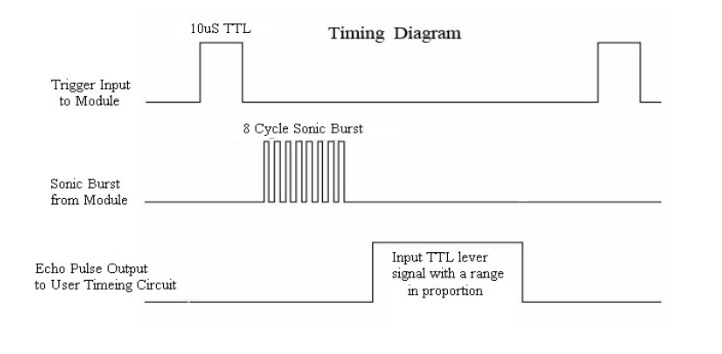
\includegraphics[width=0.7\linewidth]{Figuras/ultrasonico}
		\caption{Encendido del TRIGGER durante $10\mu s$}
		\label{fig:ultrasonico}
	\end{figure}
	
	
	\newpage
	\thispagestyle{fancy}
	\subsection{Displays 7 segmentos}
	La distancia umbral configurada por el usuario se visualiza en tiempo real en dos displays de 7 segmentos conectados al puerto \texttt{PORTD}, controlados mediante multiplexado utilizando los pines \texttt{RC2} y \texttt{RC3}. Se desarrolló una rutina cíclica que actualiza cada display con su correspondiente valor BCD convertido y codificado, permitiendo una visualización clara y estable.
	\begin{lstlisting}[caption={Multiplexado de displays}, label={lst:displays}]
		LOOP
		BSF	    PORTC,3 ; rutina para multiplexar displays
		MOVF    DISPLAY1,0
		MOVWF   PORTD
		CALL    DELAY5MS
		BCF	    PORTC,3
		BSF	    PORTC,2
		MOVF    DISPLAY2,0
		MOVWF   PORTD
		CALL    DELAY5MS
		BCF	    PORTC,2
		DECFSZ  CONTADOR3
		GOTO    LOOP
	\end{lstlisting}
	
	\subsection{Pulsador e interruptores adicionales}
	Adicionalmente, se incorporaron tres botones conectados a los pines \texttt{RB2}, \texttt{RB3} y \texttt{RB5}, los cuales permiten ejecutar funciones adicionales sin interferir con la comunicación Bluetooth. El botón en \texttt{RB2} actúa como freno de emergencia y detiene al vehículo de inmediato, mientras que los botones en \texttt{RB3} y \texttt{RB5} permiten girar hacia la izquierda y derecha, respectivamente, sin necesidad de enviar un comando desde el celular.
	\begin{lstlisting}[caption={Check de pulsador e interruptores}, label={lst:boton}]
		BOTON_POLL
		CALL    DELAY5MS        ; Antirrebote
		CALL    DELAY5MS
		CALL    DELAY5MS
		CALL    DELAY5MS
		BTFSS   PORTB, 2        ; Verifico si sigue presionado
		
		GOTO    BOTON_ACCION    ; Si, ejecuto accion
		BTFSS   PORTB, 3
		GOTO    BOTON_IZQ
		BTFSS   PORTB, 5
		GOTO    BOTON_DER
		GOTO    CONTINUAR       ; No, fue un rebote
		
		BOTON_IZQ
		CALL    IZQUIERDA            ; Izquierda
		MOVLW   'I'
		MOVWF   ESTADO_MOVIMIENTO
		MOVWF   DATO_RX
		GOTO    CONTINUAR
		
		BOTON_DER
		CALL    DERECHA            ; Derecha
		MOVLW   'D'
		MOVWF   ESTADO_MOVIMIENTO
		MOVWF   DATO_RX
		GOTO    CONTINUAR
		
		BOTON_ACCION
		CALL    STOP            ; Detengo motores
		MOVLW   'S'
		MOVWF   ESTADO_MOVIMIENTO
		MOVWF   DATO_RX
		
		CONTINUAR
		RETURN
	\end{lstlisting}
	\newpage
	\thispagestyle{fancy}
	El sistema se encuentra diseñado para funcionar de forma robusta, con rutinas antirrebote por software, manejo eficiente de interrupciones por recepción serial y temporización precisa para la medición ultrasónica. Todo el comportamiento del sistema está gestionado mediante estados definidos en registros internos, que permiten mantener el último comando recibido y restaurarlo cuando sea necesario.
	
	\section{Diagrama circuital}
	En la sección a continuación se detalla un diagrama circuital obviando las resistencias y los transistores utilizados para simplificar el entendimiento del mismo. Por otro lado, las salidas de control de los motores están representadas como LEDS.
	\begin{figure}[h!]
		\centering
		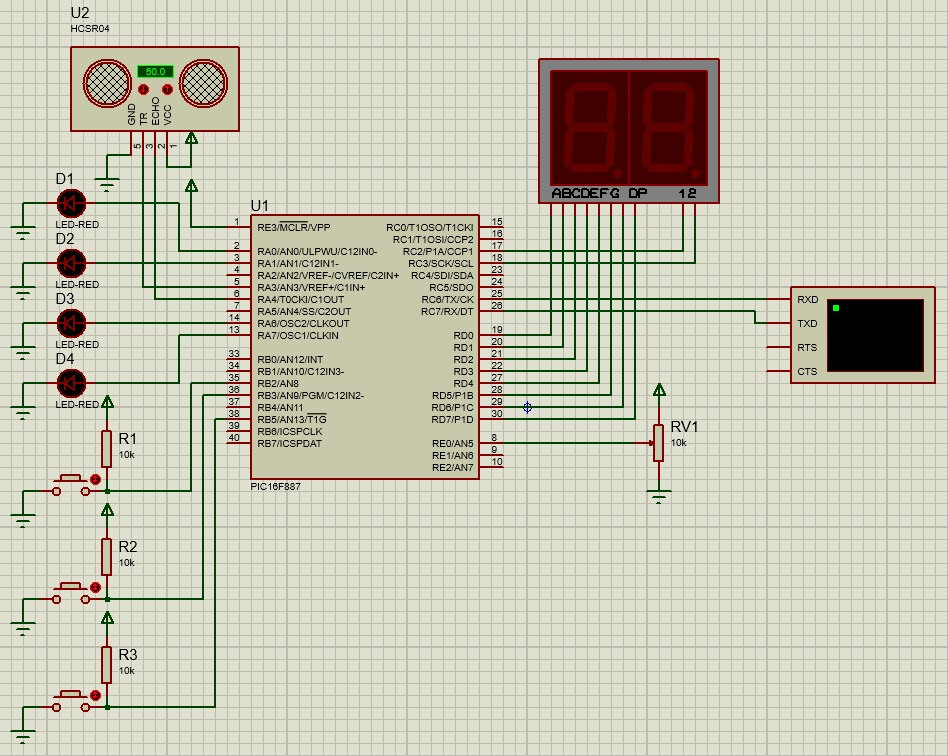
\includegraphics[width=0.7\linewidth]{Figuras/diagrama_circuital}
		\caption{Diagrama circuital}
		\label{fig:diagramacircuital}
	\end{figure}
	
	\section{Fragmentos relevantes del código}
	
	A continuación se presentan las secciones más significativas del código desarrollado para el funcionamiento del auto. Cada fragmento ha sido seleccionado por su importancia funcional y se acompaña de una breve explicación.
	
	\newpage
	\thispagestyle{fancy}
	
	\subsection{Inicialización de periféricos}
	
	\begin{lstlisting}[caption={Configuración de puertos, ADC, USART, variables}, label={lst:config}]
		CONF
		BANKSEL ANSEL
		CLRF    ANSEL   ; seleccion puertos digitales y analogicos
		CLRF    ANSELH
		
		BANKSEL OSCCON
		movlw   b'01100000'	    ;Oscilador interno a 4 MHz	
		movwf   OSCCON
		
		; Configurar RE0 como entrada
		BANKSEL TRISE
		BSF     TRISE, 0        ; RE0 como entrada
		
		; Habilitar AN5 (RE0) como canal analogico
		BANKSEL ANSEL
		BSF     ANSEL, 5        ; AN5 habilitado
		
		BANKSEL PORTE
		CLRF    PORTE
		
		BANKSEL TRISA
		MOVLW   b'10110000'	; RC7/RX entrada
		MOVWF   TRISC	; RC6/TX salida
		; Y PARA MULTIPLEXAR DISPLAYS
		MOVLW   b'00100100'	; configuracion USART
		MOVWF   TXSTA	; y activacion de transmision
		MOVLW   .25		; 9600 Baudios
		MOVWF   SPBRG
		BSF	    PIE1,RCIE	; Habilita interrupcion en recepcion
		CLRF    TRISA
		BCF	    TRISA,3 ; TRIGGER = SALIDA
		BSF	    TRISA,4 ; ECHO = ENTRADA
		CLRF    TRISD   ; PUERTO D DISPLAY
		CLRF    TRISB
		BSF	    TRISB, 2 ; RB2 --> INPUT
		BSF	    TRISB, 3 ; RB3 --> INPUT
		BSF	    TRISB, 5 ; RB5 --> INPUT
		
		BANKSEL RCSTA
		MOVLW   b'10010000'	; configuracion del USART para recepcion continua
		MOVWF   RCSTA		; puesta en ON
		
		BANKSEL OPTION_REG	; configuracion timer 0
		MOVLW   B'00000000'
		MOVWF   OPTION_REG
		
		BANKSEL ADCON0
		MOVLW   b'00010101'    ; Canal AN5, ADC encendido
		MOVWF   ADCON0
		
		BANKSEL ADCON1
		MOVLW   b'00000000'   
		MOVWF   ADCON1
		
		MOVLW   b'11000000'	; Habilitacion de las interrupciones en general
		MOVWF   INTCON
		
		BANKSEL PORTC   ; limpio registros que voy a utilizar
		BCF	    TRIGGER ; APAGO TRIGGER
		CLRF    PORTA
		CLRF    PORTB
		CLRF    PORTC
		CLRF    PORTD
		CLRF    W
		CLRF    CONT0
		CLRF    ESTADO_MOVIMIENTO
		CLRF    DATO_RX
		MOVLW   'S'
		MOVWF   ESTADO_MOVIMIENTO
	\end{lstlisting}
	
	\newpage
	\thispagestyle{fancy}
	
	Este bloque configura los puertos analógicos, la comunicación serie (USART), el ADC, y activa las interrupciones necesarias.
	
	\subsection{Subrutina de interrupción}
	\begin{lstlisting}[caption={Subrutina de interrupción}, label={lst:isr}]
		ISR ; rutina de interrupcion
		BTFSC   PIR1,RCIF	; Interrupcion por recepcion?
		GOTO    RECEPCION  ; Si --> voy a decodificar dato recibido
		BTFSS   INTCON,2	; Interrupcion por tmr0?
		GOTO    FINALIZAR	; No --> termina ISR
		MOVLW   TMR0_CARGA58  ; mientras el echo sea 0 las interrupciones estaran 
		MOVWF   TMR0          ; habilitadas y se repetira la recarga de tmr0 hasta
		INCF    VAR_DISTANCIA ; que se termine la medicion
		BCF	    INTCON,2
		RETFIE
	\end{lstlisting}
	
	\subsection{Control de motores}
	
	\begin{lstlisting}[caption={Rutina para avanzar}, label={lst:adelante}]
		ADELANTE
		BCF	PORTA,0
		BCF	PORTA,1
		BCF	PORTA,6
		BCF	PORTA,7
		BSF	PORTA,1
		BSF	PORTA,7
		RETURN
	\end{lstlisting}
	
	El control del movimiento se realiza fijando los niveles adecuados en los pines de los motores. Rutinas para retroceder, girar y detenerse son análogas a la mostrada.
	
	\subsection{Lectura de distancia con sensor ultrasónico}
	
	\begin{lstlisting}[caption={Inicio de medición ultrasónica}, label={lst:ultrasonico}]
		START 
		BCF     PIR1, RCIF
		CLRF    VAR_DISTANCIA
		BSF     TRIGGER
		CALL    DELAY_10_MICROS
		BCF     TRIGGER
	\end{lstlisting}
	
	Se genera un pulso de 10 microsegundos en el pin \texttt{TRIGGER} y se mide el tiempo hasta recibir el eco haciendo uso del \texttt{TIMER0}.
	
	\subsection{Lectura del umbral desde potenciómetro}
	
	\begin{lstlisting}[caption={Lectura del valor de frenado}, label={lst:adc}]
		LECTURA_ADC
		BANKSEL ADCON0
		BSF     ADCON0, GO
		ADC_WAIT
		BTFSC   ADCON0, GO
		GOTO    ADC_WAIT
		MOVF    ADRESH, W
		MOVWF   DISTANCIA_UMBRAL
		RETURN
	\end{lstlisting}
	
	El valor leído del ADC representa la distancia mínima antes de frenar automáticamente, el valor se guarda en la variable DISTANCIA UMBRAL.
	
	\newpage
	\thispagestyle{fancy}
	
	\subsection{Visualización en displays}
	
	\begin{lstlisting}[caption={Multiplexado de displays de 7 segmentos}, label={lst:display}]
		LOOP
		BSF     PORTC,3
		MOVF    DISPLAY1,0
		MOVWF   PORTD
		CALL    DELAY5MS
		BCF     PORTC,3
		
		BSF     PORTC,2
		MOVF    DISPLAY2,0
		MOVWF   PORTD
		CALL    DELAY5MS
		BCF     PORTC,2
		
		DECFSZ  CONTADOR3
		GOTO    LOOP
	\end{lstlisting}
	
	Este fragmento actualiza los valores visualizados en los displays de forma alternada para generar el efecto de multiplexado.
	
	\subsection{Frenado por botón físico}
	
	\begin{lstlisting}[caption={Frenado de emergencia}, label={lst:boton}]
		BOTON_ACCION
		CALL    STOP
		MOVLW   'S'
		MOVWF   ESTADO_MOVIMIENTO
		MOVWF   DATO_RX
	\end{lstlisting}
	
	Ante la activación de un botón físico conectado a RB2, el sistema detiene los motores y guarda el nuevo estado como `'S'` (Stop).
	
	\section{Pruebas, problemas y resultados}
	
	Para validar el correcto funcionamiento del sistema desarrollado, se llevaron a cabo una serie de pruebas funcionales sobre cada uno de los subsistemas implementados. Estas pruebas se realizaron sobre el prototipo final, alimentado con una batería de $9\,V$.
	
	\subsection{Pruebas de movimiento por Bluetooth}
	
	Se utilizaron comandos enviados desde la aplicación \texttt{LightBlue} para verificar los desplazamientos del vehículo en las cuatro direcciones posibles. Se comprobó que el sistema responde correctamente a los comandos \texttt{‘A’} (adelante), \texttt{‘R’} (retroceso), \texttt{‘I’} (izquierda) y \texttt{‘D’} (derecha), enviando las señales apropiadas a los pines de control de los motores. Se observó una respuesta inmediata al recibir cada comando, y la dirección se mantiene hasta recibir una nueva orden o activarse alguna condición de frenado.
	
	\subsection{Frenado automático por proximidad}
	
	Con el sensor ultrasónico ubicado en la parte delantera del vehículo, se midió la distancia a obstáculos colocados en su trayectoria. Se utilizó un potenciómetro para configurar la distancia mínima de frenado, la cual se visualiza en tiempo real en los displays. Cuando el obstáculo se encuentra a una distancia menor que la configurada, el sistema detiene automáticamente el movimiento del vehículo, y se mantiene detenido hasta que el obstáculo se retira. Al tener únicamente 2 displays se tomó como máxima distancia los $99\,cm$, pero de acuerdo al datasheet la distancía máxima de medición es mayor ($400\,cm$).
	
	\newpage
	\thispagestyle{fancy}
	
	\subsection{Visualización en displays}
	
	Los displays de 7 segmentos muestran el valor del umbral de frenado leído por el ADC. Se comprobó que el valor cambia en tiempo real al girar el potenciómetro. La multiplexación garantiza una visualización estable, con leves parpadeos debido a las múltiples mediciones.
	
	\subsection{Interacción con pulsador e interruptores físicos}
	
	Se probaron tres botones conectados a los pines \texttt{RB2}, \texttt{RB3} y \texttt{RB5}. El botón en \texttt{RB2} cumple la función de freno de emergencia, deteniendo el movimiento del vehículo y sobrescribiendo el estado anterior. Los botones en \texttt{RB3} y \texttt{RB5} permiten girar a la izquierda o a la derecha sin necesidad de utilizar el celular. Todos los botones cuentan con una rutina antirrebote por software que evita activaciones no deseadas.
	
	\subsection{Resumen de resultados}
	
	El sistema respondió correctamente a prácticamente todo lo esperado, y se comprobó que es capaz de:
	
	\begin{itemize}
		\item Ejecutar órdenes de movimiento de forma remota con mínima latencia.
		\item Frenar automáticamente al detectar obstáculos, de acuerdo con un umbral configurable.
		\item Detenerse con un pulsador de emergencia.
		\item Visualizar correctamente la distancia de frenado en los displays.
		\item Realizar giros laterales utilizando botones físicos.
	\end{itemize}
	
	Se concluye que el comportamiento del sistema es robusto y cumple con los objetivos propuestos.
	
	\subsection{Problemas}
	
	Durante el desarrollo e implementación del proyecto se presentaron distintos inconvenientes tanto a nivel de hardware como de software. A continuación se detallan los problemas de mayor relevancia, junto con las estrategias adoptadas para su resolución.
	
	\subsubsection{1. Consumo de energía y comportamiento errático de los motores}
	
	Uno de los primeros problemas observados fue el comportamiento inestable del vehículo durante las pruebas prolongadas. Los motores no respondían de forma adecuada, deteniéndose, no arrancando, apagando todos los componentes o mostrando pérdida de potencia. Este comportamiento fue atribuido al rápido desgaste de las baterías utilizadas, debido a los picos de corriente producidos por los motores al momento de arrancar y frenar.
	
	\textbf{Solución:} Se sustituyó la batería agotada por una batería de pruebas durante el desarrollo, y se reservó una batería nueva y completamente cargada exclusivamente para la presentación final. Esta medida permitió asegurar el funcionamiento estable del sistema en todo momento.
	
	\subsubsection{2. Fallas en la lectura de botones}
	
	Inicialmente se proyectó la utilización de un teclado matricial como método de entrada adicional para controlar funciones del vehículo sin necesidad de Bluetooth. Sin embargo, su implementación presentó múltiples dificultades:
	
	\begin{itemize}
		\item El teclado interfería con las pruebas de movilidad, al dificultar el acceso físico al prototipo en movimiento.
		\item Las interrupciones por cambio de estado en el puerto \texttt{PORTB} no permitían el funcionamiento del teclado matricial.
		
		\newpage
		\thispagestyle{fancy}
		
		\item Se observaron comportamientos erráticos incluso con interrupciones por flanco en el pin \texttt{RB0}.
	\end{itemize}
	
	Se realizaron numerosas pruebas para intentar resolver el problema, entre ellas:
	
	\begin{itemize}
		\item Reemplazo del teclado por botones individuales y/o interruptores.
		\item Variación del tipo de interrupción: cambio de estado, flanco de bajada y flanco de subida.
		\item Utilización de distintos pines del puerto \texttt{PORTB} (desde \texttt{RB0} hasta \texttt{RB7}).
		\item Soldado de cables directamente a los pines del pulsador.
		\item Verificación del correcto funcionamiento de los botones con un multímetro (continuidad y caída de tensión).
		\item Pruebas con resistencias de pull-up internas del microcontrolador, y con resistencias externas conectadas manualmente.
	\end{itemize}
	
	A pesar de todos los intentos, no se logró un funcionamiento estable utilizando interrupciones. Las resistencias de pull-up internas del PIC \texttt{16F887} no funcionaron adecuadamente con los botones implementados, lo cual agravaba la situación. También se realizó una simulación en Proteus, cuyo resultado está detallado en un vídeo en la sección "Anexo".
	
	\textbf{Solución:} Finalmente se descartó el uso de interrupciones para la lectura de botones, y se optó por una verificación por \textbf{polling} durante el ciclo principal del programa. Esta técnica permitió una detección robusta del estado de los botones, acompañada de una rutina antirrebote por software (antirrebote realizado a partir de la rutina de delay ya configurada) para evitar falsas activaciones.
	
	\section{Montaje}
	
	En la sección a continuación se muestran diferentes imágenes donde se puede observar desde diferentes perspectivas el montaje del auto:
	
	\newpage
	\thispagestyle{fancy}
	
	\begin{figure}[h!]
		\centering
		\begin{subfigure}[b]{0.45\textwidth}
			\centering
			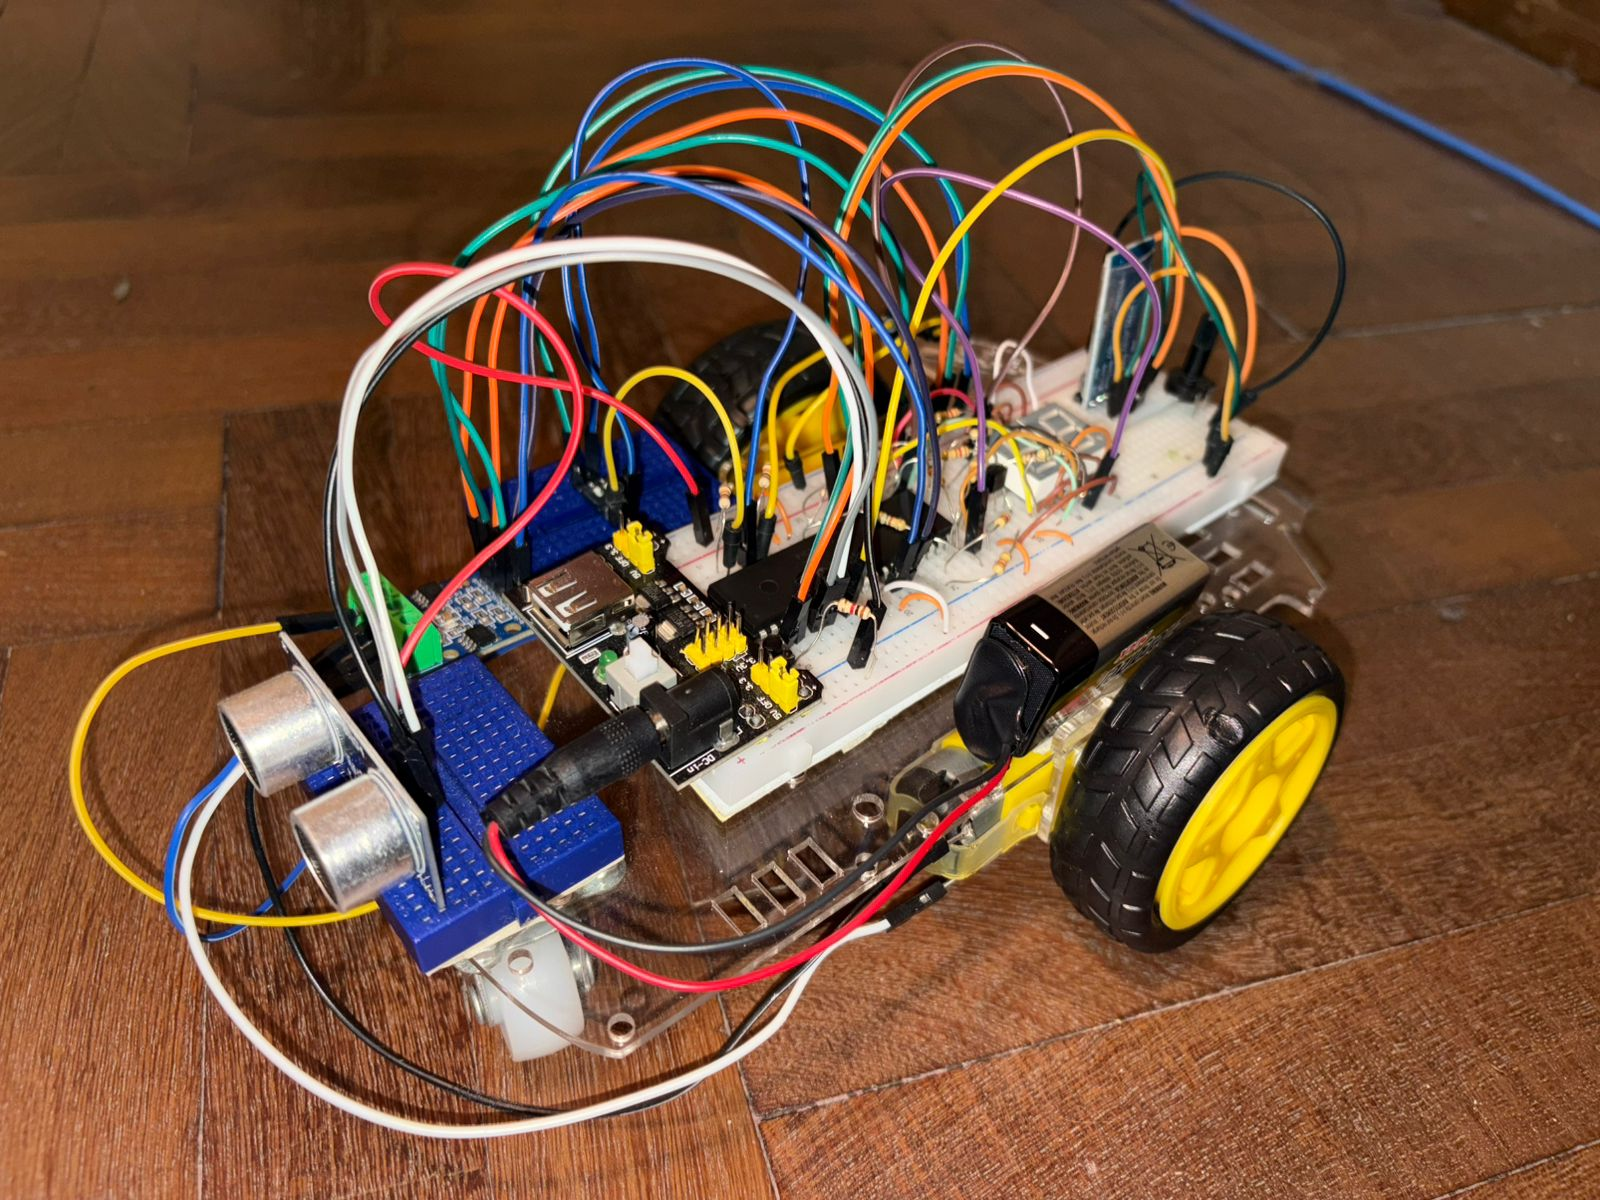
\includegraphics[width=\linewidth]{Figuras/montaje_1}
			\caption{Montaje del circuito - vista 1}
			\label{fig:montaje1}
		\end{subfigure}
		\hfill
		\begin{subfigure}[b]{0.45\textwidth}
			\centering
			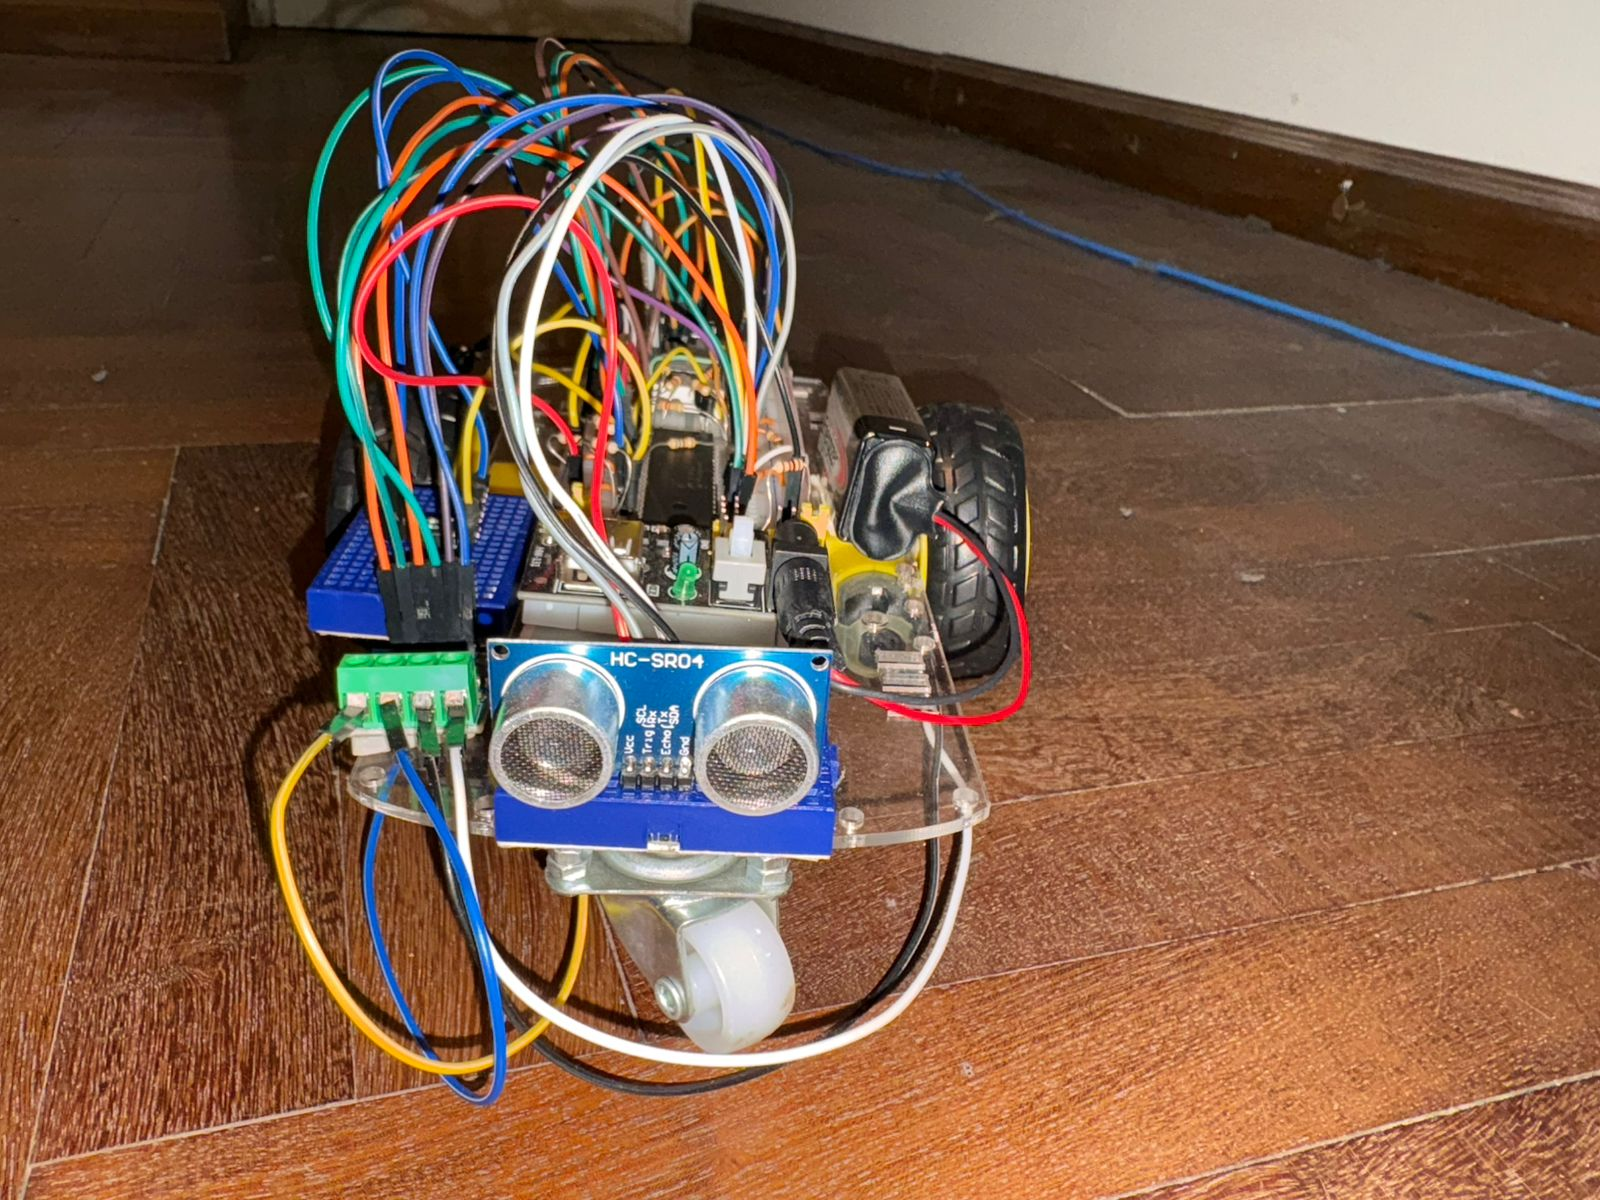
\includegraphics[width=\linewidth]{Figuras/montaje_2}
			\caption{Montaje del circuito - vista 2}
			\label{fig:montaje2}
		\end{subfigure}
		
		\vspace{0.5cm}
		
		\begin{subfigure}[b]{0.45\textwidth}
			\centering
			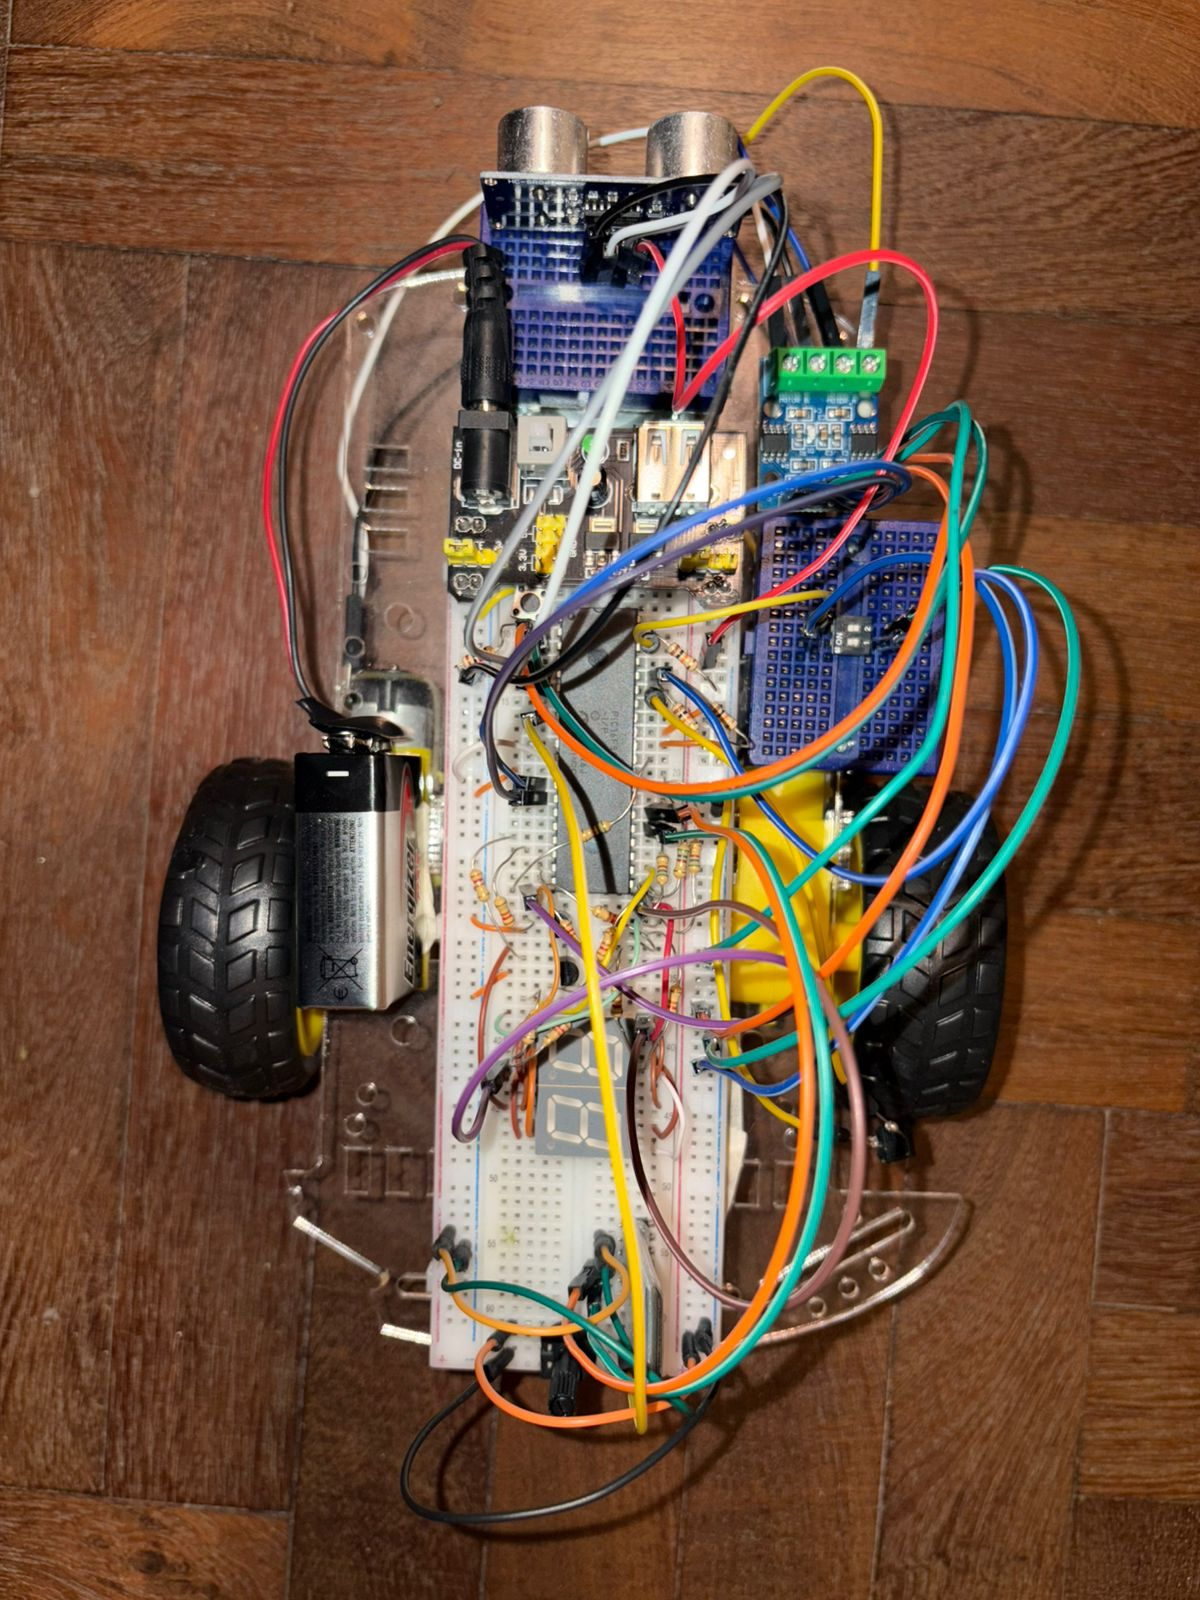
\includegraphics[width=\linewidth]{Figuras/montaje_3}
			\caption{Montaje del circuito - vista 3}
			\label{fig:montaje3}
		\end{subfigure}
		\hfill
		\begin{subfigure}[b]{0.45\textwidth}
			\centering
			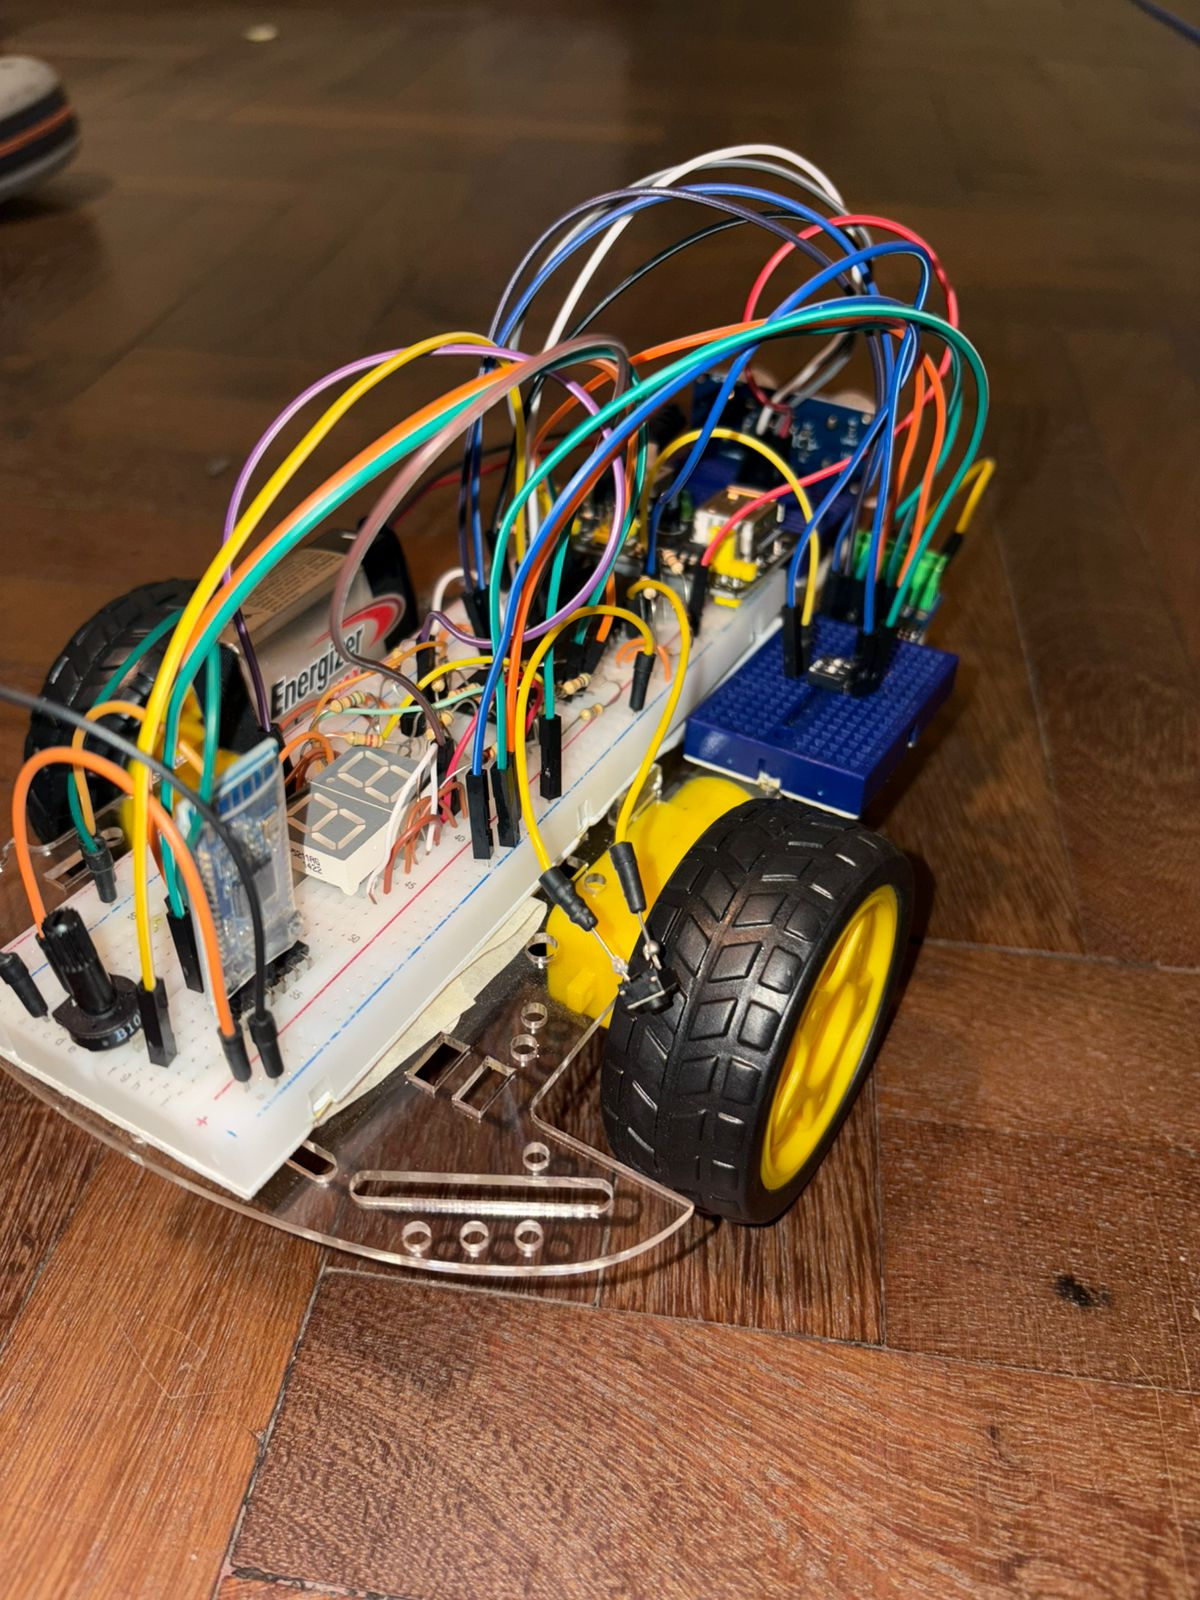
\includegraphics[width=\linewidth]{Figuras/montaje_4}
			\caption{Montaje del circuito - vista 4}
			\label{fig:montaje4}
		\end{subfigure}
		
		\caption{Montaje físico del sistema en distintos ángulos.}
		\label{fig:montaje_completo}
	\end{figure}
	
	\section{Conclusiones}
	
	El desarrollo del presente proyecto permitió integrar diversos conocimientos adquiridos a lo largo de la asignatura, aplicándolos en un sistema funcional. El vehículo \textbf{Terreneitor} se mostró de amplia utilidad para la experimentación y uso de las diferentes funcionalidades del microcontrolador \texttt{PIC16F887}, tales como el módulo ADC, TIMER0, USART, interrupciones y técnicas de multiplexado.
	
	Se logró implementar un sistema que opera por un lado, mediante comunicación Bluetooth desde un celular, y por otro, mediante botones físicos que permiten la operación directa del vehículo.
	
	La inclusión del sensor ultrasónico y del potenciómetro como entrada al ADC permitió simular una funcionalidad de “frenado automático” configurable por el usuario, lo cual añade una capa de complejidad y automatización al comportamiento del robot. 
	
	Asimismo, el uso de displays de 7 segmentos controlados por multiplexado permitió una visualización en tiempo real del umbral de frenado, haciendo el sistema más comprensible para el usuario.
	
	\newpage
	\thispagestyle{fancy}
	
	A pesar de los desafíos encontrados, particularmente en la implementación del botón, las soluciones adoptadas permitieron alcanzar un sistema estable y funcional. En definitiva, este proyecto permitió consolidar habilidades en diseño digital, programación de un microcontrolador \texttt{PIC16F887}, análisis de hardware, y resolución de problemas de integración electrónica.
	
	\newpage
	\appendix
	\section{Anexo - Repositorio y documentación técnica}
	
	\subsection{Repositorio del proyecto}
	
	El código fuente completo del trabajo práctico final, así como imágenes y documentación adicional (vídeo de simulación interrupción con botón), se encuentran disponibles en el siguiente repositorio (de mi propiedad) público de GitHub:
	
	\begin{itemize}
		\item \href{https://github.com/EsqueletinhoX/Trabajo_Final_Digital_2/tree/main}{\texttt{github.com/EsqueletinhoX/Trabajo\_Final\_Digital\_2}}
	\end{itemize}
	
	\vspace{1cm}
	
	\subsection{Hojas de datos de componentes}
	
	A continuación, se listan las hojas de datos (datasheets) correspondientes a los principales componentes utilizados en el desarrollo del proyecto:
	
	\begin{itemize}
		\item \textbf{Sensor ultrasónico HC-SR04:} \href{https://www.alldatasheet.com/datasheet-pdf/view/1132203/ETC2/HC-SR04.html}{alldatasheet.com/datasheet/HC-SR04}
		\item \textbf{Módulo Bluetooth BLE (basado en CC2541):} \href{https://www.alldatasheet.com/datasheet-pdf/view/454131/TI/CC2541.html}{alldatasheet.com/datasheet/CC2541}
		\item \textbf{Regulador de tensión AMS1117:} \href{https://www.alldatasheet.com/datasheet-pdf/view/49118/ADMOS/AMS1117.html}{alldatasheet.com/datasheet/AMS1117}
		\item \textbf{Transistor BC547:} \href{https://www.alldatasheet.com/datasheet-pdf/view/11551/ONSEMI/BC547.html}{alldatasheet.com/datasheet/BC547}
		\item \textbf{Microcontrolador PIC16F887:} \href{https://www.alldatasheet.com/datasheet-pdf/view/197543/MICROCHIP/PIC16F887.html}{alldatasheet.com/datasheet/PIC16F887}
		\item \textbf{Display 7 segmentos:}
		\href{https://www.alldatasheet.com/datasheet-pdf/view/819442/LIGHTKEY/LD5211AG.html}{alldatasheet.com/datasheet/7SEG}
	\end{itemize}
	
	
\end{document}